% Autor: Leonhard Segger, Alexander Neuwirth
% Datum: 2017-10-30
\documentclass[
	% Papierformat
	a4paper,
	% Schriftgröße (beliebige Größen mit „fontsize=Xpt“)
	12pt,
	% Schreibt die Papiergröße korrekt ins Ausgabedokument
	pagesize,
	% Sprache für z.B. Babel
	ngerman
]{scrartcl}

% Achtung: Die Reihenfolge der Pakete kann (leider) wichtig sein!
% Insbesondere sollten (so wie hier) babel, fontenc und inputenc (in dieser
% Reihenfolge) als Erstes und hyperref und cleveref (Reihenfolge auch hier
% beachten) als Letztes geladen werden!

\usepackage{tikz}
\usetikzlibrary{calc,patterns,angles,quotes} % loads some tikz extensions\usepackage{tikz}
\usetikzlibrary{babel}

% Silbentrennung etc.; Sprache wird durch Option bei \documentclass festgelegt
\usepackage{babel}
% Verwendung der Zeichentabelle T1 (Sonderzeichen etc.)
\usepackage[T1]{fontenc}
% Legt die Zeichenkodierung der Eingabedatei fest, z.B. UTF-8
\usepackage[utf8]{inputenc}
% Schriftart
\usepackage{lmodern}
% Zusätzliche Sonderzeichen
\usepackage{textcomp}

% Mathepaket (intlimits: Grenzen über/unter Integralzeichen)
\usepackage[intlimits]{amsmath}
% Ermöglicht die Nutzung von \SI{Zahl}{Einheit} u.a.
\usepackage{amssymb}
% mehr symbole plox
\usepackage{siunitx}
% Zum flexiblen Einbinden von Grafiken (\includegraphics)
\usepackage{graphicx}
% Abbildungen im Fließtext
\usepackage{wrapfig}
% Abbildungen nebeneinander (subfigure, subtable)
\usepackage{subcaption}
% Funktionen für Anführungszeichen
\usepackage{csquotes}
\MakeOuterQuote{"}
% Zitieren, Bibliografie
\usepackage[sorting=none]{biblatex}
% "\vcentcolon" für := und =:
\usepackage{mathtools}


% Zur Darstellung von Webadressen
\usepackage{url}
%chemische Formeln
\usepackage[version=4]{mhchem}
% siunitx: Deutsche Ausgabe, Messfehler getrennt mit ± ausgeben
\usepackage{floatrow}
\floatsetup[table]{capposition=top}
\usepackage{float}
% Verlinkt Textstellen im PDF-Dokument
\usepackage[unicode]{hyperref}
% "Schlaue" Referenzen (nach hyperref laden!)
\usepackage{cleveref}
\sisetup{
	locale=DE,
	separate-uncertainty
}
\bibliography{References}

\begin{document}

	\begin{titlepage}
		\centering
		{\scshape\LARGE Versuchsbericht zu \par}
		\vspace{1cm}
		{\scshape\huge Mirkowellen - Bauelemente und stehende Wellen in Koaxialkabeln \par}
		\vspace{2.5cm}
		{\LARGE Gruppe BA-C-04 \par}
		\vspace{0.5cm}

		{\large Alexander Neuwirth (E-Mail: a\_neuw01@wwu.de) \par}
		{\large Leonhard Segger (E-Mail: l\_segg03@uni-muenster.de) \par}
		\vfill

		durchgeführt am 01.07.2019\par
		betreut von\par
		{\large Dr. Johann Jersch} %TODO fine so?

		\vfill

		{\large \today\par}
	\end{titlepage}
	\tableofcontents
	\newpage


	\section{Kurzfassung}
	% Hypothese	und deren Ergebnis, wenn Hypothese ist, dass nur Theorie erfüllt, sagen: Erwartung: Theorie aus einführung (mit reflink) erfüllt
	% Ergebnisse, auch Zahlen, mindestens wenn's halbwegs Sinn ergibt
	% Was wurde gemacht
	% manche leute wollen Passiv oder "man", manche nicht

  \section{Theorie}
	% wdh. Texte
	% wdh. Besprechung

	%Dezibel-Gedöns würde ich weglassen. Ist eigentlich basic.

	\subsection{Leitungstheorie} %TODO vlt. ist die Überschrift komisch, weil das alles Leitungstheorie ist.

	Bei transversalelektromagnetischen Leitern (welche im folgenden verwendet werden) lassen sich die Größen der elektromagnetischen Felder auf die einfacher zu handhabenden Größen Strom und Spannung reduzieren.
	In \cref{fig_ersatzschaltbild} ist das Ersatzschaltbild eines Abschnittes eines TEM-Leiters dargestellt.
	Ein TEM-Leiter besteht immer aus Hin- und Rückleitung.
	Die Größen der vier auftretenden Impedanzen sind abhängig von der Länge des betrachteten Leitungsabschnittes.

	\begin{figure}[H]
		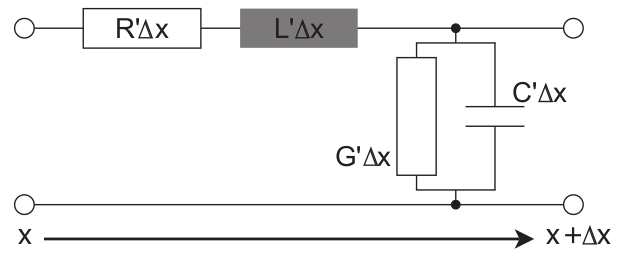
\includegraphics[width=0.8\textwidth]{img/ersatzschaltbild}
		\centering
		\caption{
			Ersatzschaltbild eines Leitungsabschnittes eines transversalelektromagnetischen Leiters. \cite{Anleitung}
		}
		\label{fig_ersatzschaltbild}
		\centering
	\end{figure}

	Aufstellen der Gleichungen für Maschen- und Knotenregel (vgl. \cite{Anleitung} ) führt zur Übertragungsfunktion:
	\begin{align}
		U(x) &= U_h \cdot e^{-\gamma x} + U_r \cdot e^{\gamma x}\\
		I(x) &= I_h \cdot e^{-\gamma x} - I_r \cdot e^{\gamma x}\\
		\text{mit} \quad \gamma \vcentcolon &= \sqrt{(R'+i \omega L')(G' +i \omega C')} = \alpha + i \beta
	\end{align}
	Dabei ist $\alpha $ der Dämpfungskoeffizient.

	\subsection{Leitungsabschluss}
	Wenn an einem Kabelende keine Reflexionen auftauchen sollen, muss der Reflexionskoeffizient verschwinden.
	Dieser ist definiert als:
	\begin{equation}
		r = \frac{Z_a-Z_L}{Z_a+Z_L} %TODO iirc war die Gleichung falsch (+- getauscht) und ist so richtig. ergibt auch Sinn.
	\end{equation}
	Dabei ist der  Leitungswiderstand
	\begin{equation}
		Z_L=\sqrt{\frac{L'}{C'}}.
	\end{equation}
	Der Abschlusswiderstand $Z_a$ soll also gleich zum Leitungswiderstand sein.

	Beim Reflexionskoeffizient entspricht $r=-1=1 \cdot e^{i\pi}$ einem Phasensprung von $\pi$.

	\subsection{Stehende Wellen}

	Stehende Wellen zeichnen sich dadurch aus, dass sie Knotenpunkte besitzen, an denen der Ausschlag stets Null ist und deren Position zeitlich konstant ist.
	Sie treten bei vollständiger Reflexion, also $| r | < 1	$, an eienr Barriere auf.

	Bei Betrachtung einer verlustlosen Leitungder Länge $l$, die an beiden Enden vollständig reflektiert, ergibt sich für die transmittierte Leistung die Airy-Funktion:

	\begin{align}
		P_t = \frac{|U_h|^2}{Z_L} \cdot \left( \frac{T}{1-R} \right) ^2 \cdot \frac{1}{1+F \sin^2 \left( \frac{\phi}{2} \right) } \\
		\text{mit dem Finesse-Faktor} \quad F= \frac{4R}{(1-R)^2} \\
		\text{und} \quad R = |r_1 ||r_2 |, \quad T= |t_1||t_2|,
	\end{align}
	wobei $t_{1,2}$ und $r_{1,2}$ die Reflexions- bzw. Transmissionskoeffizienten an den Leitungsenden sind.

	Diese wird maximal für
	\begin{equation}
		\label{eq_inter}
	\sin ^2 \left( \frac{\phi}{2} \right) = 0 \Rightarrow 2k_nl -\varphi_1 - \varphi_2 = 2\pi n,
	\end{equation}
	wobei $\varphi_1, \varphi_2 $ die Phasensprünge an den beiden Enden der Leitung sind und $n \in \mathbb{Z}$.

	\subsection{Lecherleitung und Koaxialleitung}
	Bei der Lecherleitung verlaufen Feldlinien des elektromagnetischen Feldes weit außerhalb des Leiters und führen so zu erhöhtem Leitungswiderstand und erlauben ein Einkoppeln von Außen in die Übertragung.
	In einer Koaxialleitung wird dies dadurch, dass eine Leitung innerhalb der anderen verläuft minimiert.
	Der Vergleich ist in \cref{fig_lecherkoaxial} dargestellt.


	\begin{figure}[H]
        \centering
        \begin{subfigure}[b]{0.55\textwidth}
            \centering
            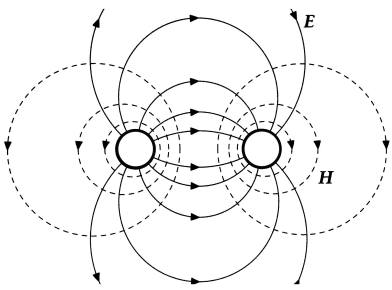
\includegraphics[width=\textwidth]{img/lecher}
            \caption{
							Lecherleitung
						}
            \label{fig_lecher}
        \end{subfigure}
        \hfill
        \begin{subfigure}[b]{0.40\textwidth}
            \centering
            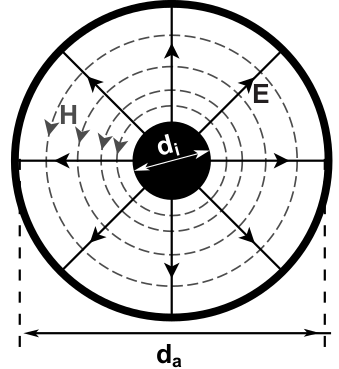
\includegraphics[width=\textwidth]{img/koaxial}
            \caption{
						Koaxialleitung
						}
            \label{fig_koaxial}
        \end{subfigure}

        \caption{Vergleich zwischen dem Verlauf der Feldlinien bei Lecher- und Koaxialleitung. \cite{Anleitung}}
				\label{fig_lecherkoaxial}
	\end{figure}


	\subsection{Mikrostreifenleitung}

	Wenn Mikrowellenleitungen auf Platinen verbaut werden sollen, ist die Koaxialleitung unpraktikabel.
	Hier kommt die Mikrostreifenleitung zum Einsatz, die, wie in \cref{fig_mikrostreifen} dargestellt, aus einem Leiter, der durch ein Dielektrikum von einer leitenden Fläche getrennt wird, besteht.
	Dies ist eine Kompromisslösung, da sie außerhalb verlaufende Feldlinien besitzt.

	\begin{figure}[H]
		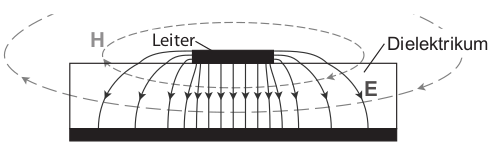
\includegraphics[width=0.8\textwidth]{img/mirkostreifen}
		\centering
		\caption{
			Verlauf der Feldlinien bei einer Mikrostreifenleitung. \cite{Anleitung}
		}
		\label{fig_mikrostreifen}
		\centering
	\end{figure}


	\subsection{Richtkoppler}

	In \cref{fig_richtkoppler} ist das Prinzip eines Richtkopplers dargestellt.
	Dieser basiert auf konstruktiver oder destruktiver Interferenz.
	Wird angenommen, dass ein Signal über Leichtung 1 einläuft, so ist schnell festzustellen, dass das Signal über die beiden direkten Wege dieselbe Strecke zurücklegt, also keine Laufzeitdifferenz aufweist, sodass an 4 konstruktive Interferenz herrscht, das Signal also übertragen wird. %TODO erwähnen, dass das auch im Kreis laufen kann und dann destruktiv ist?
	Die übertragene Leistung hängt von der Stärke der Kopplung ab.
	Wenn andersherum ein Signal von 1 nach 3 läuft, ergibt sich ein Laufzeitunterschied von $\lambda/2$ zwischen den beiden wahrscheinlichsten (und gleichwahrscheinlichen, wenn Kopplung 1 und 2 gleich sind) Wegen.
	Dementsprechend tritt destruktive Interferenz auf.

	So ergibt sich die Funktionsweise des Richtkopplers, die Wellen, welche von 1 nach 2 laufen auf Ausgang 4 koppelt, während Wellen, die von 2 nach 1 laufen auf Ausgang 3 gekoppelt werden.

	\begin{figure}[H]
		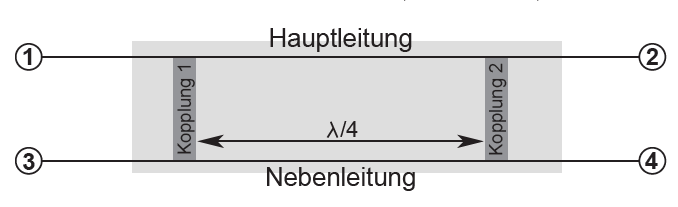
\includegraphics[width=0.8\textwidth]{img/richtkoppler.png}
		\centering
		\caption{
			Schamtische Darstellung eines Richtkopplers. Der Abstand zwischen den Kopplungen entspricht einer Weglänge von $\lambda/4$. \cite{Anleitung}
		}
		\label{fig_richtkoppler}
		\centering
	\end{figure}

	Man definiert:

	\begin{align}
		\text{Koppeldämpfung} \quad = 10 \cdot \lg{ \left( \frac{P_1}{P_4} \right) } \si{\deci \bel}
		\label{eq_koppeld}\\
		\text{Isolation} \quad = 10 \cdot \lg{ \left( \frac{P_2}{P_4} \right) } \si{\deci \bel}
		\label{eq_isolation}\\
		\text{Einfügedämpfung} \quad = 10 \cdot \lg{ \left( \frac{P_1}{P_2} \right) } \si{\deci \bel}
		\label{eq_einfueged}\\
	\end{align}

	Da die Weglängendifferenz natürlich in dieser simplifizierten Variante nur für exakt eine Frequenz passen kann, ist die Bauweise in der Realität komplexer, um eine weitere Bandbreite zuzulassen.

	\subsection{Zirkulator und Richtleitung}

	Ein Zirkulator hat, wie in \cref{fig_zirkulator} schematisch dargestellt drei Ein- bzw. Ausgänge, die jeweils in Richtung eines Ausgangs transmittieren und in Richtung des anderen isolieren.
	Dies wird herbeigefürt, indem ein dielektrisches Material mit doppelbrechenden Eigenschaften für die Transmission der Wellen verwendet wird.
	Dann wird Interferenz ausgenutzt, um an je einem Ausgang konstruktive und am anderen destruktive Interferenz zu erzeugen.

	Man definiert für für die drei Eingänge jeweils:
	\begin{align}
		\text{Durchlassdämpfung} \quad = 10 \cdot \lg{ \left( \frac{P_1}{P_2} \right) } \si{\deci \bel}
		\label{eq_durchlassd}\\
		\text{Sperrdämpfung} \quad = 10 \cdot \lg{ \left( \frac{P_1}{P_3} \right) } \si{\deci \bel}
		\label{eq_sperrd}\\
	\end{align}

	\begin{figure}[H]
		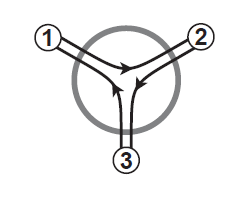
\includegraphics[width=0.3\textwidth]{img/zirkulator.png}
		\centering
		\caption{
			Schamtische Darstellung eines Zirkulators. \cite{Anleitung}
		}
		\label{fig_zirkulator}
		\centering
	\end{figure}

	Ein Isolator stellt zwischen je zwei Ausgängen eine Richtleitung da, da nur in eine Richtung laufende Wellen übertragen werden.
	Dazu muss der andere Ausgang korrekt abgeschlossen werden.
	Im Versuch wird ein 4-Tor-Zirkulator verwendet, da dieser eine höhere Rückflussdämpfung besitzt.

	\subsection{Detektordiode}

	Um Mikrowellen gleichzurichten, kann eine Diode verwendet werden.
	Deren Funktionsweise soll im Folgenden kurz beschrieben werden.

	Wenn man einen p-dotierten Halbleiter in direkten Kontakt mit einem n-dotierten bringt oder einfach einen Halbleiter an zwei Seiten unterschiedlich dotiert, nennt man dies einen pn-Übergang.

	Aus energetischen Gründen wandern dann Elektronen und Löcher aufeinander zu und rekombinieren in der Übergangszone.
	Da hierbei jedoch im n-dotierten Halbleiter Atome mit einem Elektron weniger zurückgelassen werden, als sie Protonen im Kern haben, beginnt sich auf dieser Seite des Halbleiters eine positive Gesamtladung zu sammeln.
	Gleichzeitig erhalten die Atome im p-dotierten Halbleiter ein Elektron mehr, als sie Protonen im Kern haben, sodass sich hier eine negative Gesamtladung sammelt.

	Das elektrische Feld, das durch die Ladungsdifferenz entsteht wirkt energetisch der Rekombination entgegen, sodass sich ein Gleichgewicht mit einer Raumladungszone zwischen den Halbleitern einstellt.
	Diese Raumladungszone sorgt für die vielfältigen Eigenschaften des pn-Übergangs, der als Diode fungiert:
	Wird eine Spannung so angelegt, dass der Pluspol am p-dotierten Halbleiter liegt, baut diese die Raumladungszone ab und es kommt zu einem exponentiellen Anstieg der Stromstärke.
	Wird die Spannung andersherum angelegt, wird die Raumladungszone verbreitert und die Diode sperrt, sodass der Stromfluss gering (Null) ist.

	Die Diode wird charakterisiert durch die Diodenkennlinie, die die Abhängigkeit vom Stromfluss zur angelegten Spannung angibt und idealerweise der folgenden Gleichung gehorcht:
	\begin{equation}
		\label{eq_diode_ideal}
		I = I_0 \left[ \exp \left( \frac{eU}{n k_B T} \right) -1 \right] %TODO prüfen, ob das schön ist, weil kann ich nicht
	\end{equation}


	\section{Methoden}
	% Bilder von der Website klauen
	% einer will Präsens

	\subsection{Diodenkennlinie}
	Die Diodenkennlinie der im Folgenden verwendeten Messdiode soll aufgenommen werden, um anhand der gemessenen Spannung auf die am Ausgang der verschiedenen Bauteile ankommende Leistung zurückschließen zu können.
	Dazu wird der in \cref{fig_aufbau_kennlinie} dargestellte Aufbau verwendet.
	Am Mikrowellengenerator werden verschiedene Leistungen durchgefahren und jeweils die Spannung am Ausgang der Messdiode gemessen.
	Zur Automatisierung des Messvorgangs wird ein LabView-Programm verwendet.

	\begin{figure}[H]
		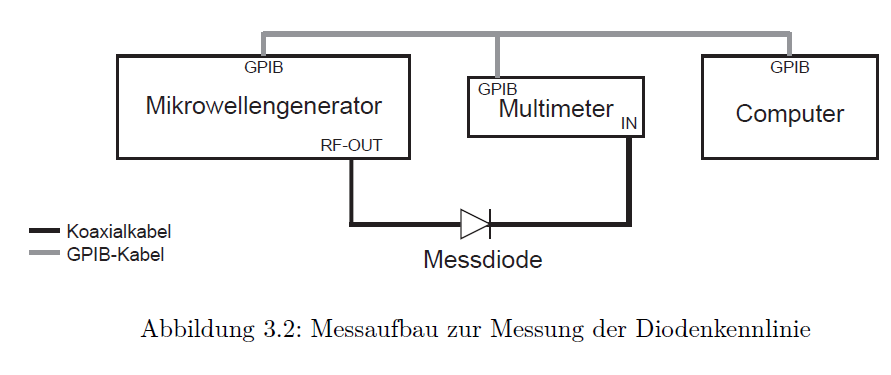
\includegraphics[width=0.8\textwidth]{img/aufbau_kennlinie.png}
		\centering
		\caption{
		 	Messaufbau zur Messung der Diodenkennlinie. \cite{Anleitung}
		}
		\label{fig_aufbau_kennlinie}
		\centering
	\end{figure}

	\subsection{Eigenschaften von Hochfrequenzbauteilen}

	Es wird der in \cref{fig_aufbau_bauteile} dargestellte Aufbau mit der zuvor vermessenen Diode verwendet.
	Dann wird für die im Folgenden genannten Bauteile Messungen auf einem jeweils etwas breiteren Frequenzband, als laut Hersteller empfohlen, durchgeführt.
  Bei den Messungen wird jeweils bei fester Eingangsleistung die Ausgangsspannung der Diode gemessen.
	Vermessen werden Isolator (Richtleitung), Richtkoppler und zwei verschiedene Zirkulatoren (jeweils nur zwischen zwei Ein- bzw- Ausgängen).

	\begin{figure}[H]
		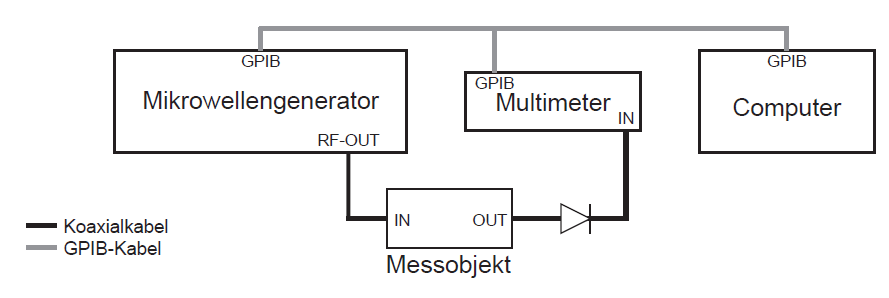
\includegraphics[width=0.8\textwidth]{img/aufbau_bauteile.png}
		\centering
		\caption{
		 	Messaufbau zur Messung der Eigenschaften verschiedener Bauteile. \cite{Anleitung}
		}
		\label{fig_aufbau_bauteile}
		\centering
	\end{figure}

	\subsection{Stehende Wellen in einem Koaxialkabel}

	Um stehende Wellen in einem Koaxialkabel zu erzeugen, wird der Aufbau in \cref{fig_aufbau_resonanzen} verwendet.
	Der Koppler wird durch eine Mirkowellenleitung realisiert, welche als Spiegel mit einer Transmittivität von \SI{1}{\percent} und einer Reflektivität von \SI{99}{\percent} (näherungsweise) fungiert.
	Die Teilwellen, welche in der Messleitung laufen, können, wenn die Weglänge der Wellen in der Messleitung einem Vielfachen ihrer Wellenlänge entspricht, dort stehende Wellen erzeugen.
	Hierbei ist anzumerken, dass streng genommen abhängig von der Art des Abschlusses ein unterschiedlicher Phasensprung $\phi$ an diesem Ende des Kabels auftritt, sodass nicht von einem Vielfachen gesprochen werden kann, sondern die Weglänge $s = n\lambda - \phi$ sein muss.
	Da jedoch in der Auswertung nur die Frequenzdifferenz zwischen den Resonanzen betrachtet wird, spielt das hier keine Rolle.

	Wann immer stehende Wellen auftreteten, kommt ausschließlich die am Koppler reflektierte Leistung an der Messdiode an, sodass die gemessene Spannung hier geringer ist, als wenn Wellen die Messleitung verlassen können.
	%TODO habe ich das richtig verstanden?

	\begin{figure}[H]
		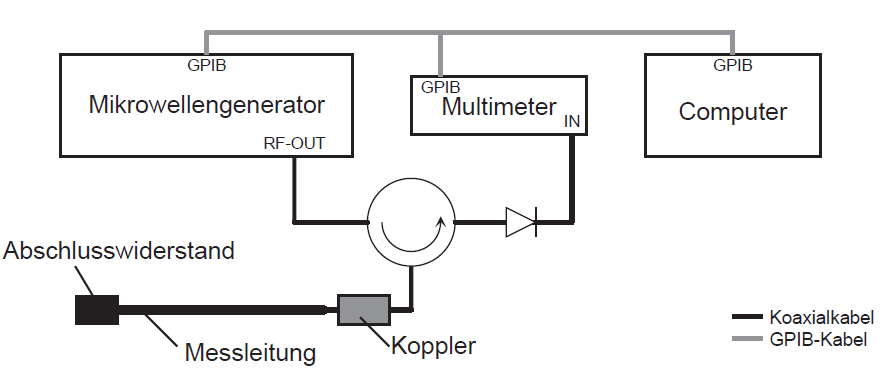
\includegraphics[width=0.8\textwidth]{img/aufbau_resonanzen.png}
		\centering
		\caption{
		 	Messaufbau zur Messung von stehenden Wellen in einem Koaxialkabel. Die Messleitung wird ohne Widerstand abgeschlossen (Kurzschluss). \cite{Anleitung}
		}
		\label{fig_aufbau_resonanzen}
		\centering
	\end{figure}

	\section{Ergebnisse und Diskussion}
	%TODO Unsicherheiten


	\subsection{Unsicherheiten}
	Alle Unsicherheiten werden nach GUM bestimmt und berechnet.
	Für diese Berechnungen wurde die Python Bibliothek \enquote{uncertainties} herangezogen, welche den Richtlinien des GUM folgt.

	\subsection{Kalibration der Detektordiode}
	% Allgemeine Beobachtungen
	% Einflüsse von veränderten Parametern auf Messung
	% Berechung nach Aufgabenstellung
	In \cref{fig_diode_kali} sind die aus verschiedenen Eingabeleistungen resultierenden Spannungen mit einer Exponentialfunktion \cref{eq_kali} angepasst worden.
	Die letzten drei Messpunkte wurden für den Fit ausgeschlossen, da diese nicht mehr der exponentiellen Natur entsprechen.
	Dementsprechend können Messwerte der Diode in diesem Bereich auch nicht mehr zuverlässig umgerechnet werden.

	\begin{equation}
		\label{eq_kali}
		U = A(e^{P/B}-C)
	\end{equation}

	\begin{figure}[H]
		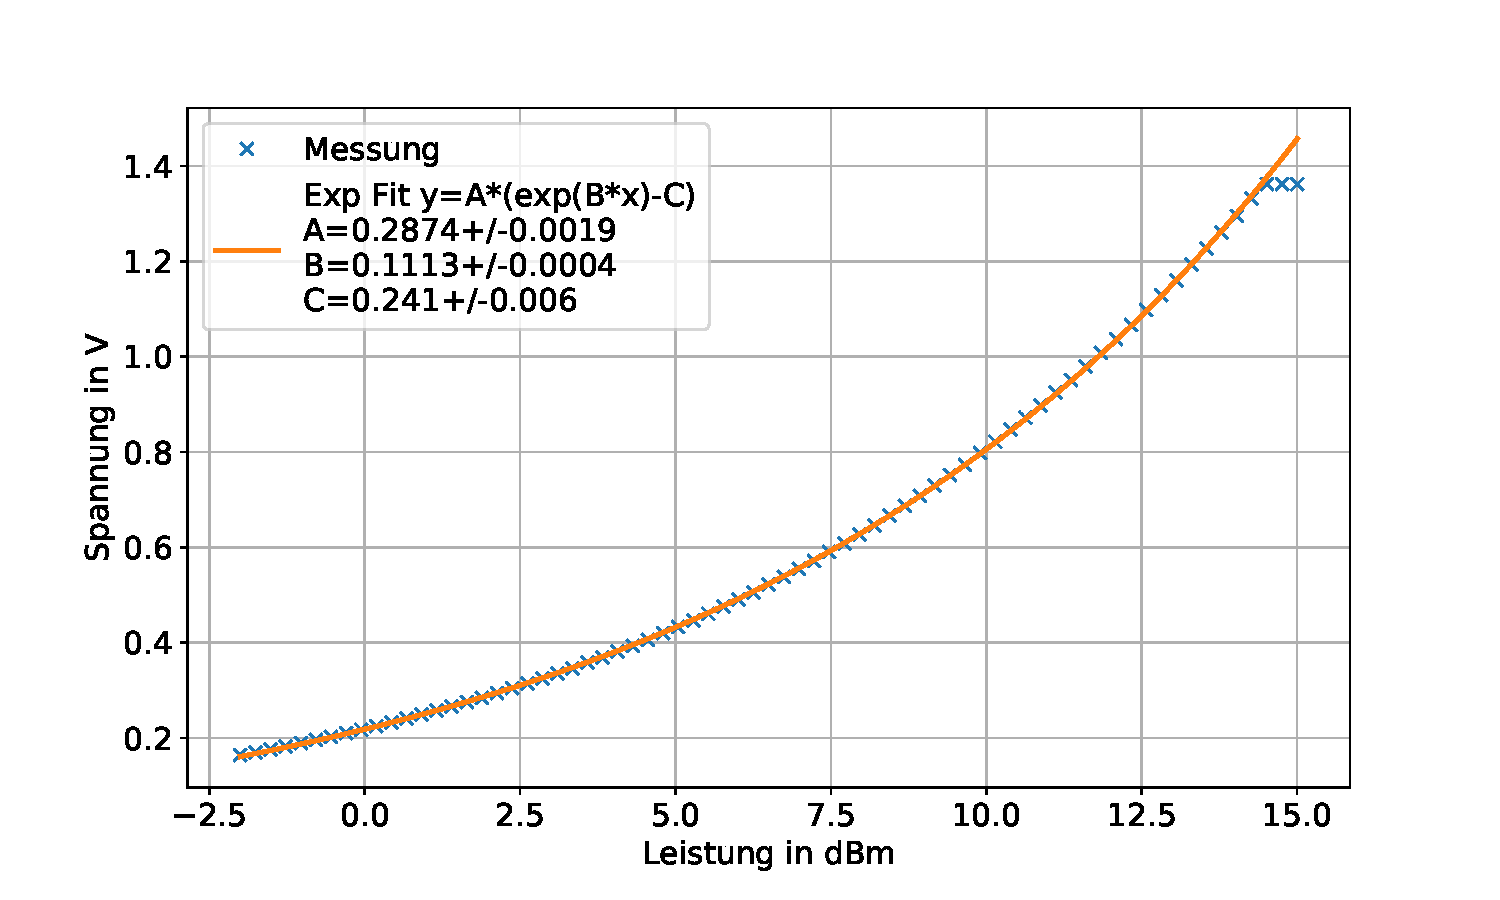
\includegraphics[width=0.8\textwidth]{img/diode-kali}
		\centering
		\caption{
			Am Multimeter gemessene Spannung bei verschiedenen Leistungen und ein exponentieller Fit nach \cref{eq_kali}.
			Die Symbole sind größer als die Unsicherheiten.
		}
		\label{fig_diode_kali}
		\centering
	\end{figure}
	Mithilfe der Inversen Exponentialfunktion \label{eq_inv_kali} lassen sich im folgenden gemessen Spannungen in eine Leistung umrechnen.

	\begin{equation}
		\label{eq_inv_kali}
		P = B\log{(U/A+C)}
	\end{equation}
	\subsubsection*{Diskussion}
	% Bezug/Nutzen oder sonst was
	% auch hier die Hypothese wiederholen
	% keine Messwerte hier, nach manchen Menschen, zumindest "direkt" erstellte Diagramme net hier, auch wenn Lesbarkeit-bla

	Wie in \cref{fig_diode_kali} ist zu erkennen, dass sich die Annahme eines exponentiellen Zusammenhangs zwischen Leistung und Spannung an der Diode bestätigen lässt.
	Wrum die drei Punkte am oberen Ende der gemessenen Leistung scheinbar horizontal verlaufen, kann nicht mit Sicherheit geklärt werden.
	Es liegt jedoch die Vermutung nahe, dass eines der Bauteile oder Messgeräte in einen Sättigungsbereich kommt, sodass die gemessene Spannung konstant wird.

	\subsection{Isolator (Richtleitung)}
	In \cref{fig_isolator} sind die gemessene frequenzabhängige Dämpfungen des Isolators in beide Richtungen abgebildet.
	Hierzu wurde die Spannung wie im vorherigen Abschnitt erläutert in eine Leistung umgerechnet.
	Die Dämpfung $\alpha$ ist
	\begin{equation}
		\alpha = 10 \cdot \lg{(P_{\text{in}}/P_{\text{out}})} \cdot \si{dB}
	\end{equation}
  mit $P_\text{in}=\SI{10}{dBm}$.
	Und es folgt mit:
	\begin{equation}
		\alpha = 10 \cdot \lg{\left(\frac{P_{\text{in}}}{P_{\text{out}}} \cdot \frac{1mW}{1mW}\right)} \cdot\si{dB}
	\end{equation}
	\begin{equation}
		\alpha = (P_\text{in} \text{[dBm]} - P_\text{out} \text{[dBm]} ) \cdot\si{dB}
	\end{equation}
	\begin{figure}[H]
		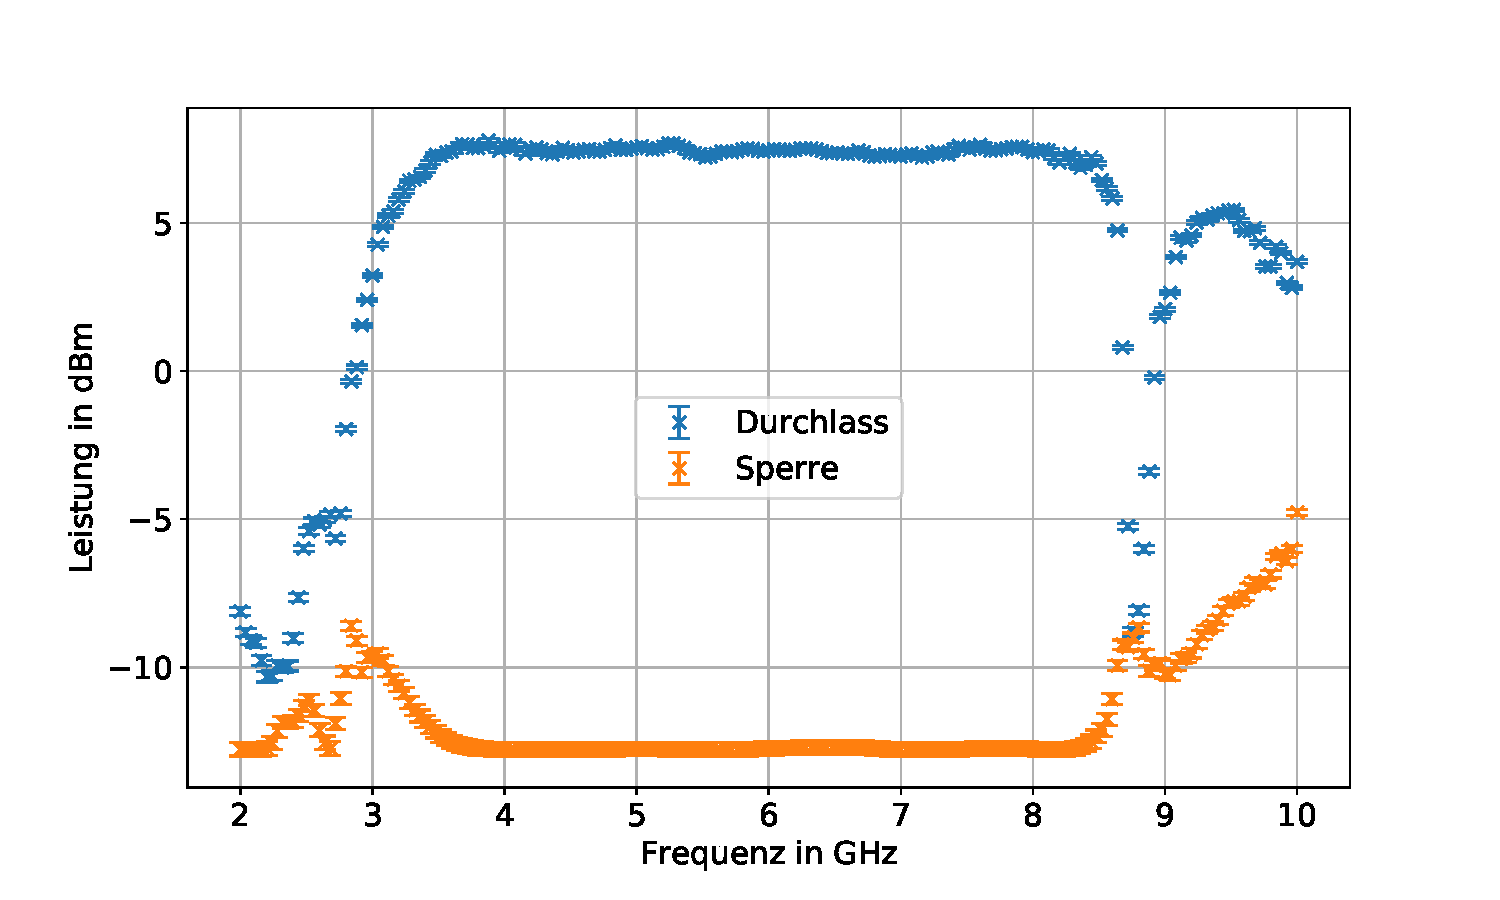
\includegraphics[width=0.8\textwidth]{img/isolator}
		\centering
		\caption{
		Durchlass- und Sperrdämpfung des Isolators in Abhängigkeit der Frequenz des Signals.
		}
		\label{fig_isolator}
		\centering
	\end{figure}
	\subsubsection*{Diskussion}
	%TODO Bandbreite Abschätzen und ggf. vergleichen mit Lit.

	Anhand von \cref{fig_isolator} soll abgeschätzt werden, welcher Frequenzbereich für die Verwendung brauchbar ist.
	Dies ist im Allgemeinen der Bereich, in dem die Durchlassdämpfung gering und die Sperrdämpfung groß ist.
	Weiterhin sollen beide Dämpfungen auch in guter Näherung konstant sein.

	Aus diesen Kriterien ergibt sich für den verwendeten Isolator (Narda 60583) ein Frequenzband von \SIrange{3,5}{8,3}{\giga \hertz}.
	Die Herstellerin gibt einen Frequenzbereich von \SIrange{3}{8,5}{\giga \hertz} an.
	Dies deckt sich zwar im Wesentlichen mit der Angabe auf Basis der Messung, bei Frequenzen sehr nahe an \SI{3}{\giga \hertz} kann jedoch anhand von \cref{fig_isolator} von einer Verwendung abgeraten werden.

	Die Herstellerin gibt außerdem an, dass im Verwendungsbereich die Einfügedämpfung unter \SI{1}{dB} und die Isolation über \SI{20}{dB} liege.
	Die erste Angabe kann widerlegt werden und die zweite trifft abgesehen von den oben genannten Frequenzen nahe \SI{3}{\giga \hertz} zu.

	\subsection{Richtkoppler}
	In analoger Weise erhält man auch die frequenzabhängigen Dämpfungen des Richtkopplers.
	Wobei $P_\text{in}$ wieder \SI{10}{dBm} ist.
	\begin{figure}[H]
		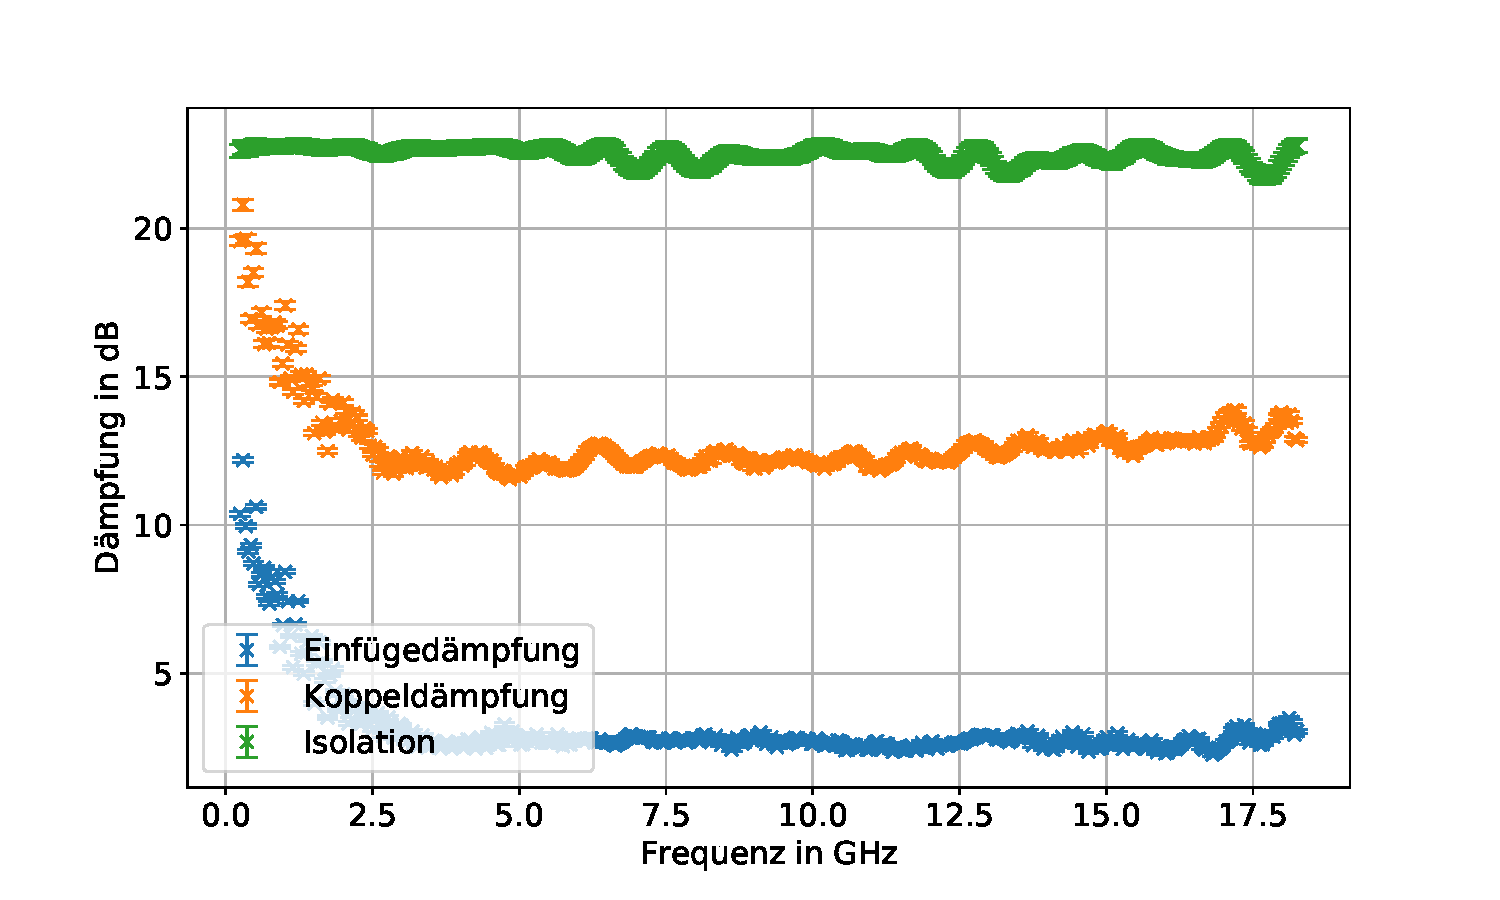
\includegraphics[width=0.8\textwidth]{img/richtkop}
		\centering
		\caption{
		Einfüge-, Koppel sowie Isolationsdämpfung des Richtkopplers in Abhängigkeit der Frequenz des Signals.
		}
		\label{fig_richt}
		\centering
	\end{figure}
	\subsubsection*{Diskussion}

	Anhand der zuvor beschriebenen Kriterien ergibt sich aus \cref{fig_richt} ein Verwendungsbereich für den Richtkoppler (Narda 4226-10) ein Frequenzbereich von \SIrange{2,6}{17,4}{\giga \hertz}.
	Die Herstellerin gibt einen Bereich von \SIrange{0,5}{18}{\giga \hertz} an, was bei geringen Frequenzen deutliche Abweichungen von der nominellen Einfüge- und Koppeldämpfung ergeben würde.
	%TODO da sind noch andere Angaben, aber die verstehe ich teilweise nicht und sie sind ultra gelogen.

	\subsection{Zirkulator}
	Ebenfalls analog ist die Bestimmung von Durchlass und Sperrdämpfung von Zirkulatoren.
	In \cref{fig_zirk} ist  $P_\text{in}=\SI{10}{dBm}$.
	\begin{figure}[H]
		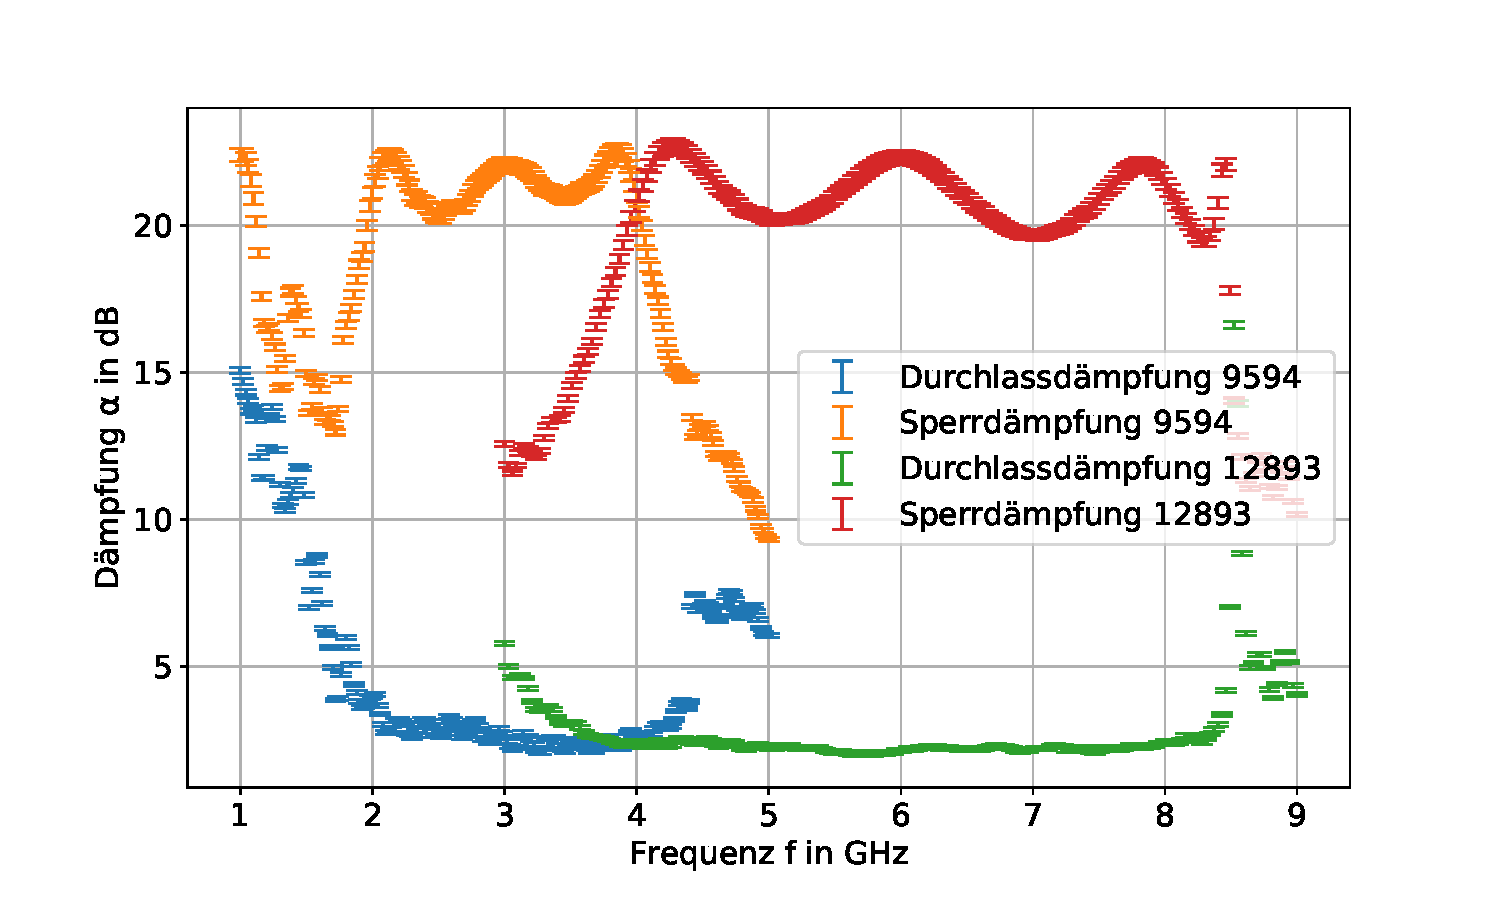
\includegraphics[width=0.8\textwidth]{img/zirkulator}
		\centering
		\caption{
	 	Durchlass- und Sperrdämpfung der vermessenen Zirkulatoren in Abhängigkeit der Frequenz des Signals.
		}
		\label{fig_zirk}
		\centering
	\end{figure}
	\subsubsection*{Diskussion}
	%TODO 9594 pass ca mit lit. Messung png
	Für den ersten Zirkulator (Modell: F61-1FFF, S/N: 9594) kann ein Verwendungsbereich von \SIrange{2}{4}{\giga \hertz} angegeben werden.
	Dies entspricht der Herstellerinnenangabe.
	Die Angabe der Sperrdämpfung mit \SIrange{20,36}{29,14}{dB} (je nach Frequenz und verwendetem Eingang) entspricht ebenfalls der Messung.
	%TODO soll insertion loss Durchlassdämpfung sein? Das passt halt nicht sehr gut.

	Für den zweiten Zirkulator (Modell: H60-1FFF, S/N: 12893) ergibt sich ein Frequenzbereich von \SIrange{4}{8,3}{\giga \hertz}, was die Herstellerinnenangabe von \SIrange{4}{8}{\giga \hertz} beinhaltet.
	Die Sperrdämpfung wird mit \SIrange{21,5}{36,08}{dB} angegeben.
	In der Messung fiel diese jedoch bis auf \SI{19,66 \pm 0,17}{dB} ab.
	%TODO Durchlassdämpfung wie oben.

	\subsection{Stehende Wellen}
	In \cref{fig_steh_well} sind die Leistungsspektren der zwei vermessenen kurzgeschlossenen Kabel aufgeführt.

	\begin{figure}[H]
        \centering
        \begin{subfigure}[b]{0.495\textwidth}
            \centering
            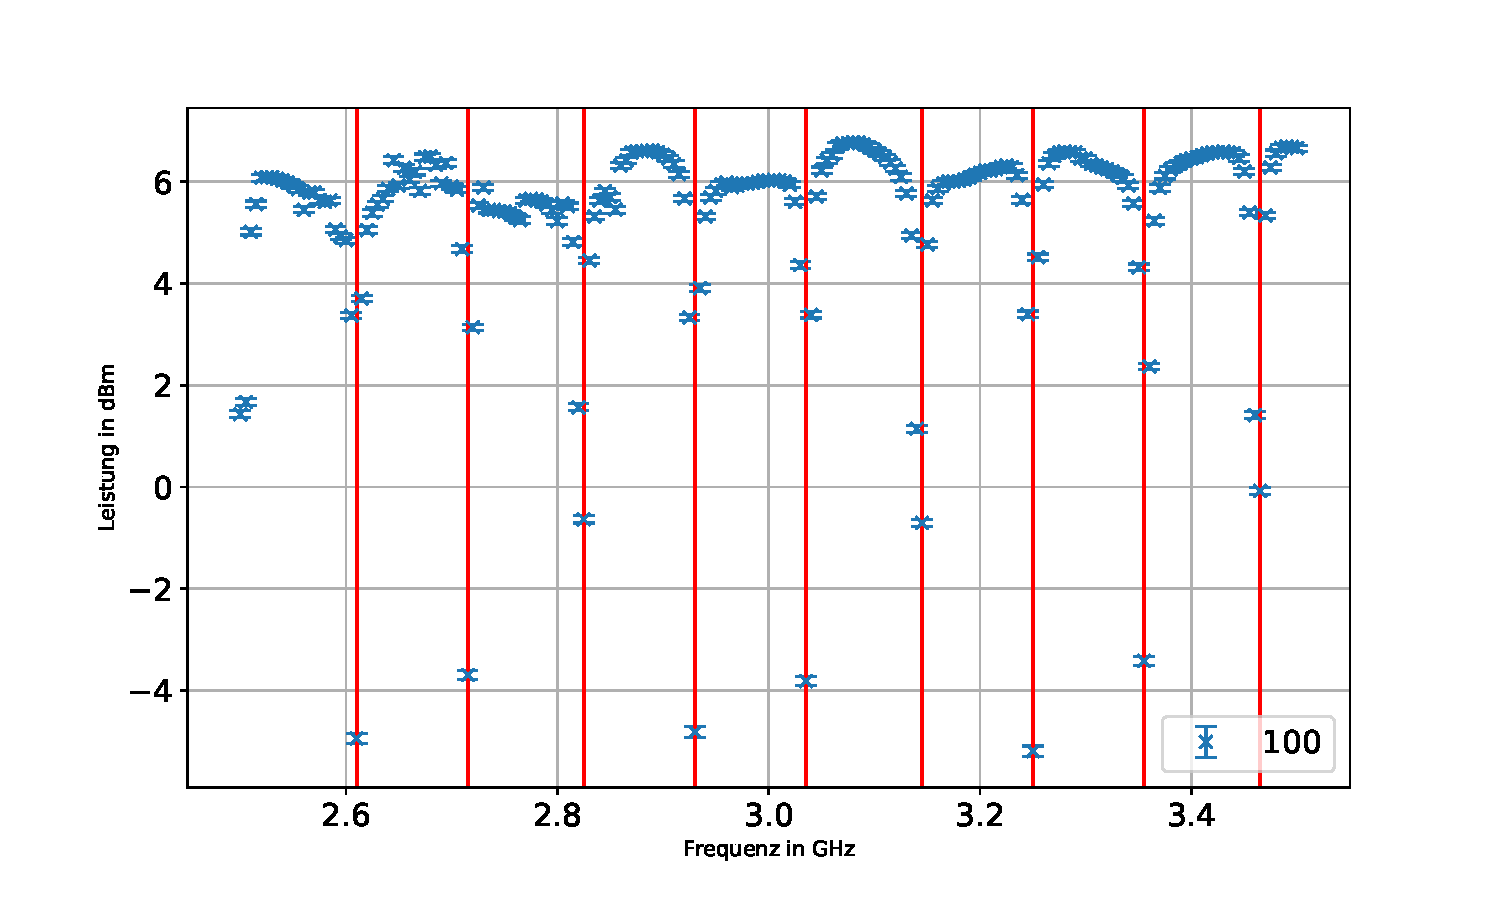
\includegraphics[width=\textwidth]{img/100}
            \caption%
            {Leistung, Kabel 1}
            \label{fig_leistung_100}
        \end{subfigure}
        \hfill
        \begin{subfigure}[b]{0.495\textwidth}
            \centering
            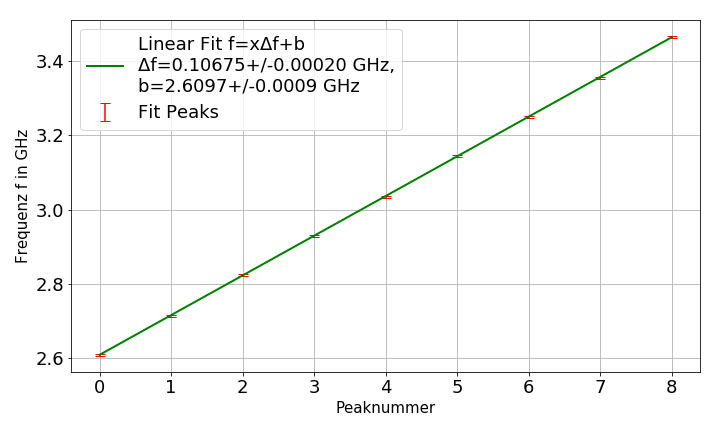
\includegraphics[width=\textwidth]{img/100_fit}
            \caption[]%
            {Fit, Kabel 1}
            \label{fig_fit_100}
        \end{subfigure}
        \begin{subfigure}[b]{0.495\textwidth}
            \centering
            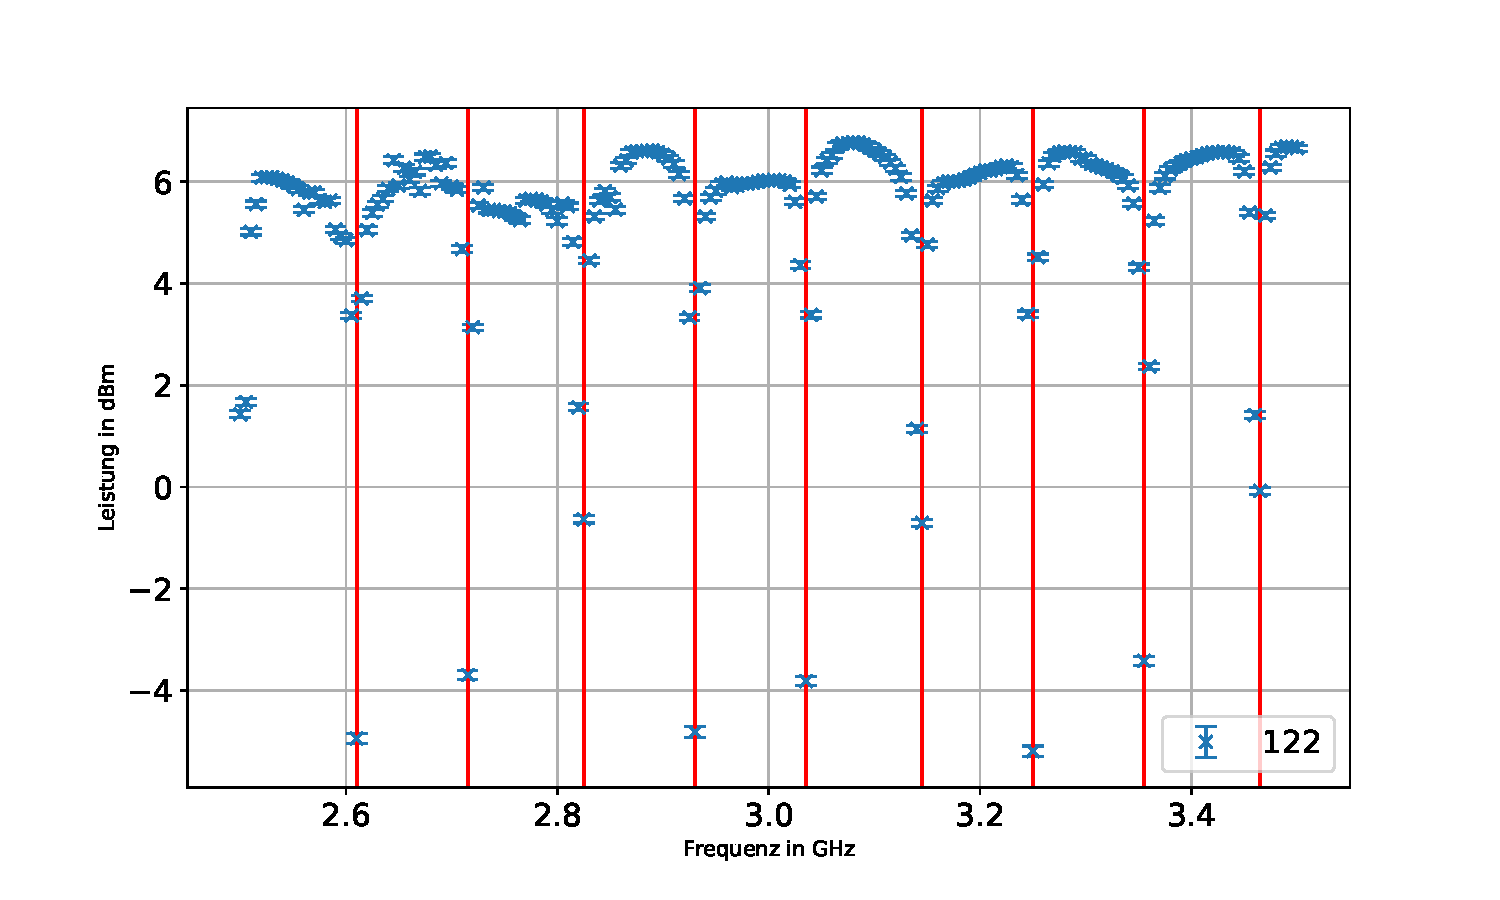
\includegraphics[width=\textwidth]{img/122}
            \caption%
            {Leistung, Kabel 2}
            \label{fig_leistung_122}
        \end{subfigure}
        \hfill
        \begin{subfigure}[b]{0.495\textwidth}
            \centering
            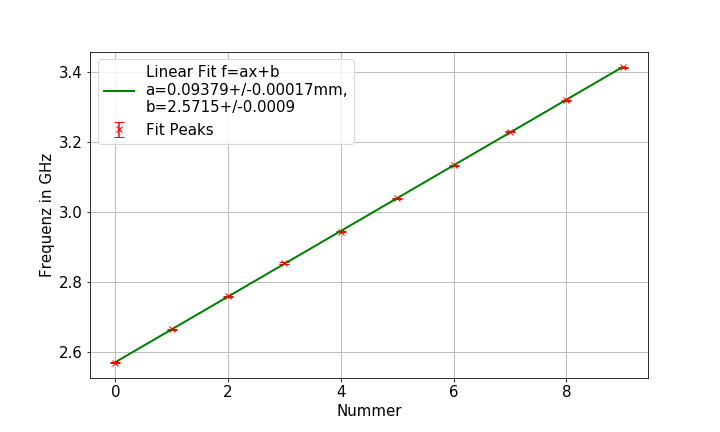
\includegraphics[width=\textwidth]{img/122_fit}
            \caption[]%
            {Fit, Kabel 2}
            \label{fig_fit_122}
        \end{subfigure}
        \caption%
        {
					Leistungsspektrum von zwei Kabeln ($l_1 = \SI{100+-1}{cm}$ und $l_2 = \SI{122+-1}{cm}$), sowie jeweilig ein Fit der Peakpositionen.
				}
        \label{fig_steh_well}
    \end{figure}

	Aus dem Abstand der Frequenzen bei denen eine Resonanz auftritt lässt sich die Ausbreitungsgeschwindigkeit im Medium bestimmen.

	\cref{eq_inter} lässt sich mittels $k_n = 2\pi f_n/c$ umschreiben zu:
	\begin{equation}
		2\pi n = l\cdot2\pi f_n /c -\phi_1 - \phi_2
	\end{equation}
	Und es folgt durch Differenzieren mit $\Delta f = f_{n+1}-f_n$:
	\begin{equation}
	c = 2l\Delta f
	\end{equation}
	Der Frequenzabstand $\Delta f$ wird durch den Fit gemittelt.
	Die Permittivitätszahl des Dielektrikums ist $\epsilon_r=(c_0/c)^2$, wobei $c_0$ die Lichtgeschwindigkeit im Vakuum ist und $\mu_r=1$ genährt wird.
	Die Ergebnisse sind in \cref{tb_res} aufgeführt.

\begin{table}[H]
	\centering
	\begin{tabular}{ c | c | c | c }
		 $l$ in \si{cm} & $\Delta f$ in \si{GHz} &  $c$ in $10^8$ \si{m/s} & $\epsilon_r$ \\ \hline
		 \input{res/tb_res}
	\end{tabular}
	\caption{
	Gemessene Länge $l$ der Kabel und Resonanzabstände $\Delta f$ sowie daraus ermittelte Ausbreitungsgeschwindigkeit $c$ und Permittivitätszahl $\epsilon_r$.
	}
	\label{tb_res}
\end{table}
	\subsubsection*{Diskussion}

	In \cref{fig_leistung_100} und \cref{fig_leistung_122} sind die Leistungsabfälle bei den Resonanzfrequenzen deutlich zu erkennen und die Auftragung der Abstände der Minima in \cref{fig_fit_100} und \cref{fig_fit_122} zeigen, dass die Abweichungen vom mittleren Abstand sehr gering sind.

	Die Berechnung der relativen Permittivitätszahlen in \cref{tb_res} zeigen, dass angenommen werden kann, dass für die Dielectrica der beiden Koaxialkabel verschiedene Materialien verwedet wurden.

	Übliche Dielectrica sind Polyethylen (fest oder schaumförmig), Teflon und Luft (mit Abstandshaltern).
	Teflon hat eine relative Permittivität von etwa \SI{2}{} \cite{Hippel}, was innerhalb der Unsicherheit der Messung für das kürzere Kabel entspricht.
	Dem anderen Kabel kann kein Material eindeutig zugeordnet werden.
	Dies spricht für ein schaumförmiges Plastik, für das sich aus Schaum und eingeschlossenem Gas eine zwischen den Permittivitäten der einzelnen Materialien liegende Permittivität ergibt.

	\section{Schlussfolgerung}
	% Rückgriff auf Hypothese und drittes Nennen dieser
	Insgesamt lässt sich sagen, dass alle Messungen erfolgreich durchgeführt werden konnten.
	So konnten die Dämpfungen verschiedener Bauteile in Abhängigkeit von der Frequenz bestimmt werden.

	% Quellen zitieren, Websiten mit Zugriffsdatum
	% Verweise auf das Laborbuch (sind erlaubt)
	% Tabelle + Bilder mit Beschriftung
	\printbibliography
\end{document}
